\documentclass[aps,prd,twocolumn,10pt,superscriptaddress,nofootinbib,longbibliography,floatfix]{revtex4-2}

\usepackage{amsmath,amssymb,amsfonts}
\usepackage{bm}
\usepackage{graphicx}
\usepackage{xcolor}
\usepackage{hyperref}
\graphicspath{{figures/}}
\hypersetup{colorlinks=true,linkcolor=blue,citecolor=blue,urlcolor=blue}

\newcommand{\dd}{\mathrm{d}}
\newcommand{\rt}{r_t}
\newcommand{\rp}{r_p}
\newcommand{\mb}{m_b}
\newcommand{\Eu}{E_u}

\begin{document}

\title{The Hills mechanism near a black hole in full numerical relativity:\\ Reference solutions, first runs, and the first passage (working note v1)}

\author{Track F of the numerical-relativity particle-in-cell cosmology program}

\date{Working note v1, state of 20 November 2026}

\begin{abstract}
A bound binary that passes close to a heavier black hole can be torn apart: one member is flung away and the other is captured. Near the black hole every pair of the three bodies interacts relativistically, yet the existing models of this encounter treat either all of gravity or the binary's own gravity in Newton's theory. This working note scopes a calculation of the encounter in full numerical relativity, with three moving black holes and later with binaries of collisionless clumps, and records the baseline results that precede the first full passage. Two reference solutions frame every run: the Newtonian three-body problem, which reproduces the published disruption probabilities and ejection energies, and a geodesic model in which each member follows the exact black-hole spacetime while the members attract each other in Newton's theory, which reproduces its published separation fractions and ejection speeds. At the mass ratios a full simulation can afford, between four and ten, the two references disagree in kind about which member escapes and whether one is swallowed. In full relativity, the error of the mesh dominates the constraint violation of the approximate three-black-hole data at the resolution of the passage; a light member settles to a steady coordinate speed within a few of its own masses under the weak gauge damping of the passage, while its apparent horizon drifts slowly; and a model of the code's refinement rules reproduces the mesh block by block. The first passage, at mass ratio four, starts near the capture boundary of a relativistic test mass, fits one graphics card within the allotment, and is running; its outcome decides between the two references.
\end{abstract}

\maketitle

\section{Introduction}\label{sec:intro}

A binary star that wanders close to a massive black hole is separated when the tidal field of the black hole exceeds the binding of the pair; one member leaves with a large velocity and the other stays on a bound, eccentric orbit about the black hole. This Hills mechanism explains the hypervelocity stars of the Galaxy, and its Newtonian theory is mature: in the limit of a very heavy black hole the problem reduces to the restricted parabolic three-body problem, whose disruption probability and ejection energy depend on one number, the ratio of pericentre to tidal radius \cite{Sari:2010hills,Kobayashi:2012hills,Brown:2018hills}. When the pericentre comes within a few tens of gravitational radii, relativity changes the outcome. A model that moves each member on the exact Schwarzschild spacetime and adds the Newtonian attraction between the members finds that more binaries are separated and that the ejected members move faster \cite{Manzaneda:2024geodesic}, and a study of the same encounter in Kerr spacetime calls the full problem intractable in numerical relativity \cite{Zhang:2024kerr}.

Full numerical relativity has followed three black holes of equal mass through close encounters \cite{Campanelli:2008three,Lousto:2008multiple,Heinze:2025encounters} and binaries on bound orbits about black holes four and nine times heavier, outside their tidal radius \cite{Ficarra:2024three}. A search of the literature found no calculation in which a heavier black hole separates a binary on a near-parabolic orbit with pericentre at or inside the tidal radius, and none in which a binary of matter clumps passes a black hole with all three bodies in general relativity. This track computes both with the numerical-relativity particle-in-cell method of Wu and Most \cite{Wu:2026nrpic}, rebuilt in the code AthenaK \cite{Stone:2024athenak,Zhu:2024utz}, which evolves the spacetime with moving punctures and collisionless matter with macroparticles. The work is carried out by large-language-model agents under human direction.

This note records the scoping stage, the baseline results without new code, and the set-up of the first passage:
\begin{itemize}
\item a full simulation reaches mass ratios between four and ten, where the binary must be wider than a plunge bound to be separated before its centre of mass is swallowed; the binary then meets the black hole at one to two tidal radii (Sec.~\ref{sec:problem});
\item the Newtonian reference reproduces the published disruption probabilities and energies, and the geodesic reference reproduces its published separation fractions and ejection speeds (Secs.~\ref{sec:t-newton} and \ref{sec:t-geodesic});
\item at mass ratios four and ten the two references disagree in kind: the geodesic one sends a member into the black hole, or swaps which member escapes, in most binary phases (Secs.~\ref{sec:t-scan} and \ref{sec:t-passage});
\item in full relativity the mesh dominates the constraint violation of the three-black-hole data at the passage's resolution, a light member's tracker settles quickly under the passage's weak gauge damping while its horizon drifts slowly, and a model of the refinement rules predicts the mesh (Secs.~\ref{sec:t-data}, \ref{sec:t-single} and \ref{sec:t-cost});
\item the first passage, at mass ratio four, starts near the relativistic capture boundary, runs on one card within the allotment, and decides between the references once it ends (Sec.~\ref{sec:t-p1}).
\end{itemize}
Section~\ref{sec:setup} describes the set-up and the numerical methods, and Sec.~\ref{sec:plan} the plan to the next gates and what is open. Table~\ref{tab:parameters} holds the parameters of the first passages, and Tables~\ref{tab:ledger1}--\ref{tab:ledger4} every number of the note with the registered run that produced it.

\section{The Hills problem near a black hole}\label{sec:problem}

\subsection{Scales of the encounter}\label{sec:scales}

A binary of members $m_1$ and $m_2$, total mass $\mb=m_1+m_2$ and semimajor axis $a_b$ approaches a black hole of mass $M$ on a nearly parabolic orbit of its centre of mass with pericentre $\rp$. The mass ratio is $q=M/\mb$, and we use units $G=c=1$ with $M$ as the unit of length and time. The binary is separated when the tidal acceleration of the black hole across the binary rivals the members' mutual attraction, which happens inside the tidal radius
\begin{equation}\label{eq:rt}
\rt=a_b\,q^{1/3}.
\end{equation}
The penetration factor $D=\rp/\rt$ measures how deep the binary goes. After a separation the members share the energy of the encounter: one leaves with positive energy and the other is bound to the black hole with a nearly opposite one. Their natural unit is the energy unit
\begin{equation}\label{eq:Eu}
\Eu=\frac{m_1m_2}{a_b}\,q^{1/3},
\end{equation}
the binding energy of the binary enlarged by the ratio of the tidal radius to the binary's size \cite{Sari:2010hills}. In the restricted problem, $q\to\infty$, the outcome depends only on $D$, on the orientation of the binary orbit and on its phase at pericentre.

\subsection{The plunge bound}\label{sec:plunge}

In gravitational radii, $r_g=M$ for the black hole and $r_{gb}=\mb$ for the binary, the tidal radius reads
\begin{equation}\label{eq:rtrg}
\frac{\rt}{r_g}=\frac{a_b}{r_{gb}}\,q^{-2/3}.
\end{equation}
A parabolic orbit about a Schwarzschild black hole turns around outside the black hole only if its angular momentum per unit mass exceeds $4M$; the marginally bound orbit has its pericentre at $4M$. A binary separated before its centre of mass is swallowed therefore needs $\rt>4M$, the plunge bound
\begin{equation}\label{eq:plunge}
\frac{a_b}{r_{gb}}>4\,q^{2/3}.
\end{equation}
The binary must be wide in units of its own gravitational radius, and the bound grows as the two-thirds power of the mass ratio. The members are smaller than the heavy black hole by the mass ratio and set the global time step, while the passage lasts a few hundred units of $M$, so the number of steps grows with $q$, and the reach of the method is a mass ratio of a few to ten. At $q=10$ we take $a_b=3M$, thirty gravitational radii of the binary, and at $q=4$, $a_b=5M$. The binary then shrinks by gravitational radiation on a time far longer than the passage (Table~\ref{tab:ledger1}), so its own radiation reaction plays a negligible role during the encounter.

The plunge bound concerns the centre of mass. Each member moves with the binary's internal speed in addition, which changes its angular momentum by about the pericentre times that speed, a sizeable fraction of $4M$ at the separations above. Near the separation, one member can fall below the angular momentum of the marginally bound orbit while the centre of mass stays above it. This is the origin of the plunges of Sec.~\ref{sec:t-scan}.

\subsection{Objects and observables}\label{sec:objects}

Three objects are planned: (a) a binary of two black holes passing a heavier black hole, pure vacuum, the baseline; (b) a binary of two self-gravitating collisionless clumps passing a black hole, the regime only a particle-in-cell method reaches; (c) two black holes dressed with collisionless matter. Object (a) comes first, and the first clump binary passes right after the first black-hole passage. Each passage gives whether the binary is separated, the energy given to the ejected and to the captured member, the fate of the captured member (bound, or swallowed by the black hole), the burst of gravitational waves, and for matter members their stripping and heating. One line of passages in pericentre at fixed mass ratio, for each of (a) and (b), compared with both references, is the first publishable result.

\section{Set-up and numerical methods}\label{sec:setup}

\subsection{The calculation}\label{sec:architecture}

Figure~\ref{fig:architecture} shows the parts of the calculation and their state in the released version of the code. The initial data place the binary's centre of mass at four tidal radii from the heavy black hole, in the state that the Newtonian problem reaches when started at ten tidal radii. The evolution in AthenaK moves the punctures, follows each black hole with a tracker and an apparent-horizon finder, refines the mesh around three length scales (the heavy black hole, the members, the binary orbit) and extracts the waves on spheres. Readers outside the code turn its output into trajectories, horizon masses, member energies and radiated energy, and the analysis compares them with reference models started from the same state. Several parts exist and are tested in a branch of the code or as a workaround of the track, and await a release: the mass-scaled shift damping, the common horizon of one pair, two cards for the finest resolution, a constraint solve inside the code, and clumps with momentum.

\begin{figure*}
\centering
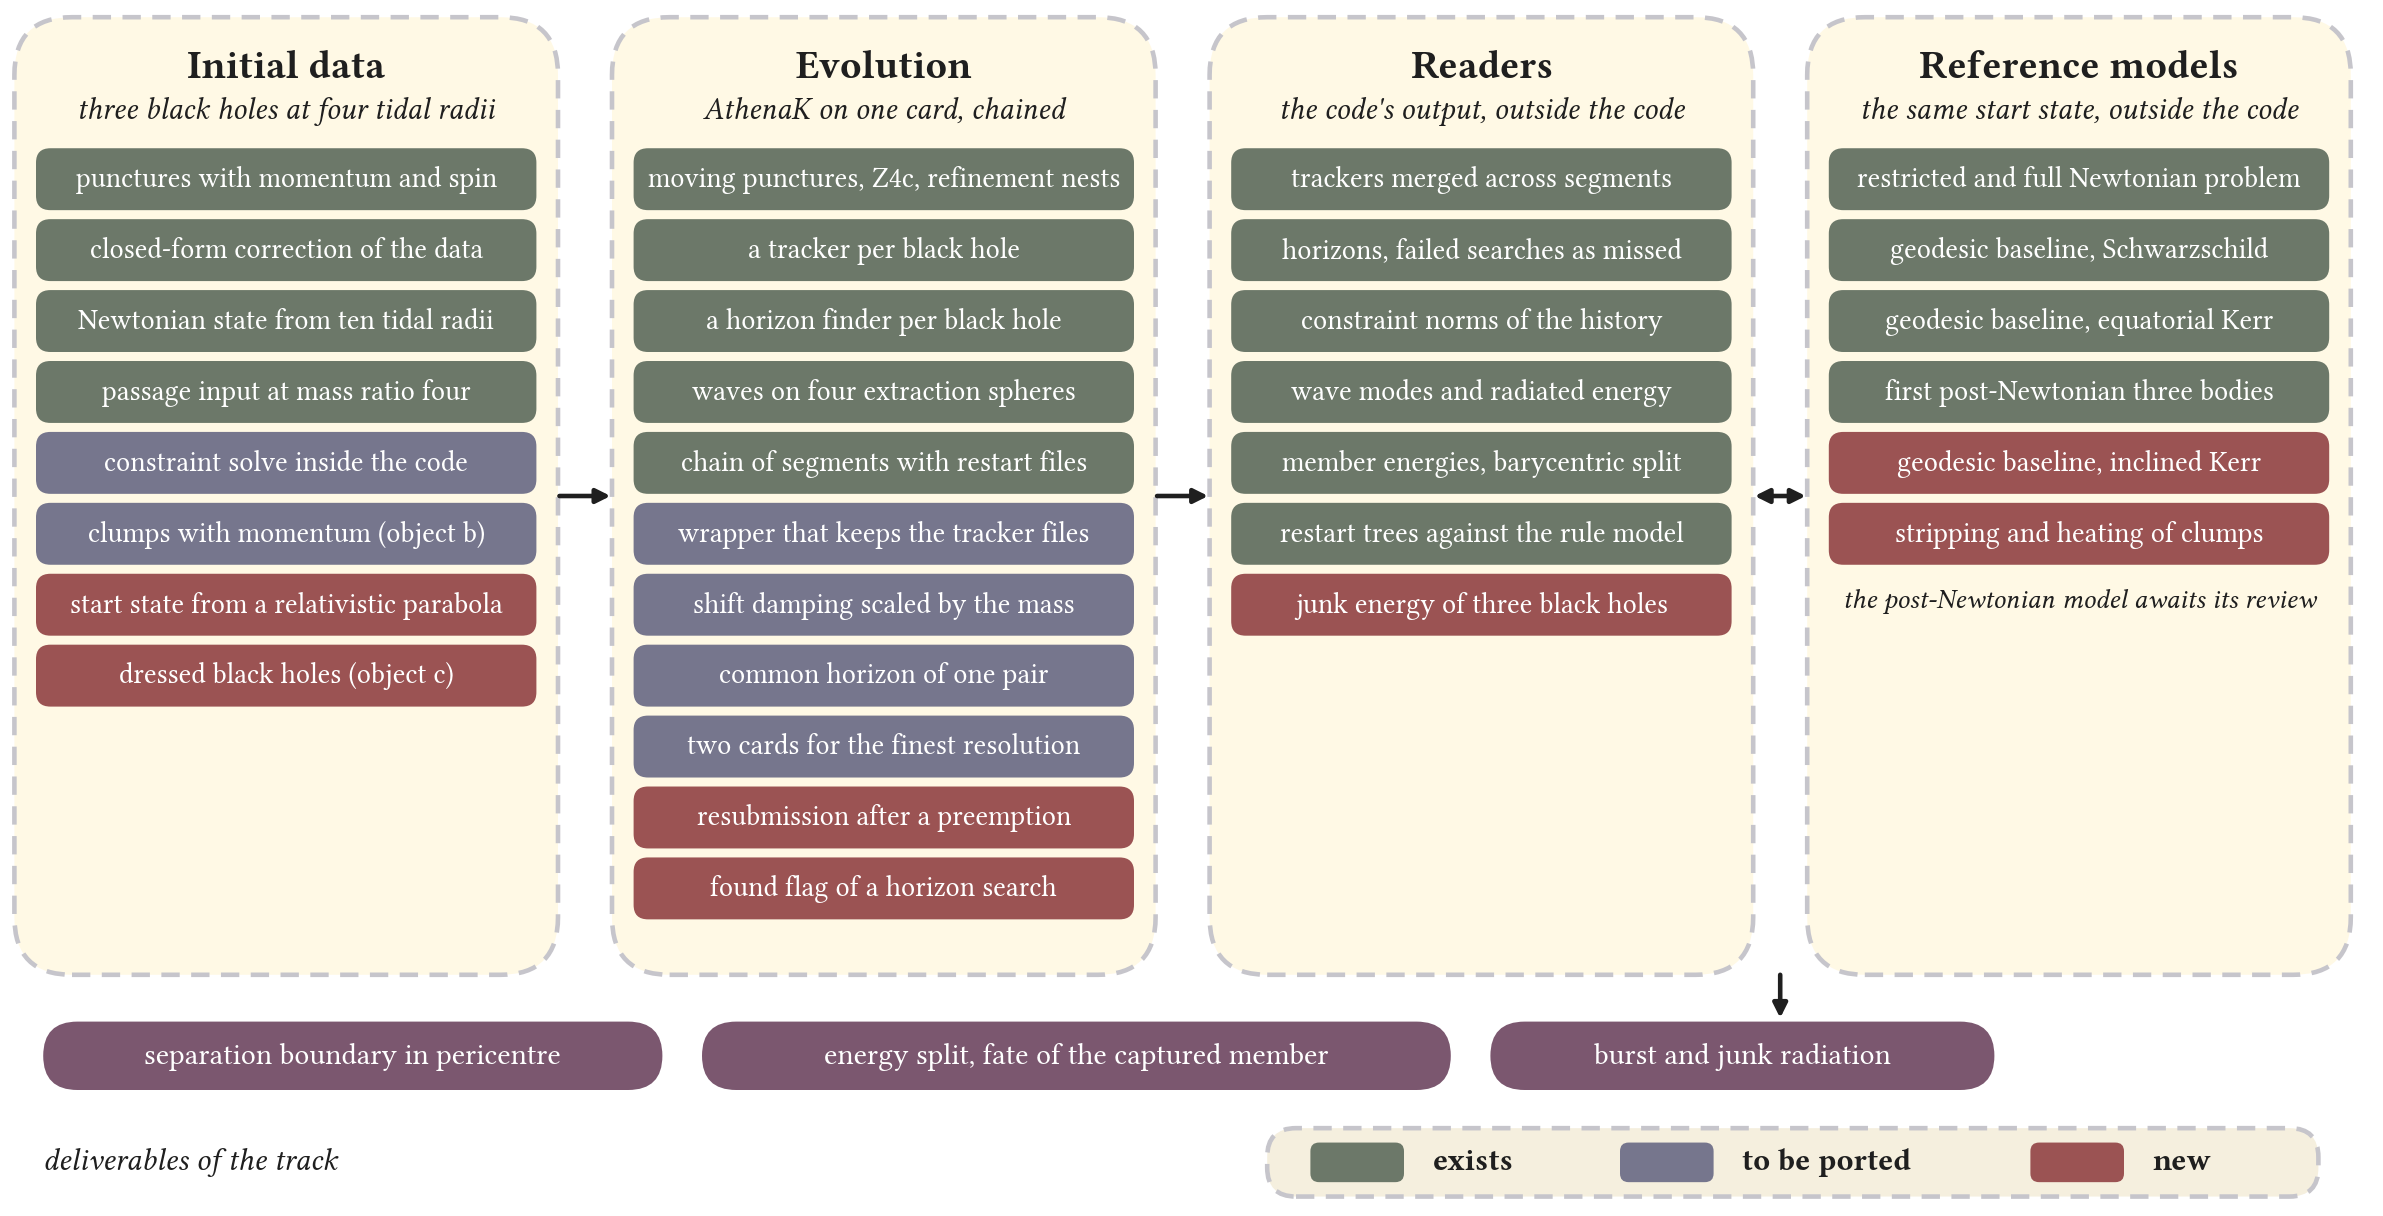
\includegraphics[width=0.94\textwidth]{schem_architecture.png}
\caption{Architecture of the calculation in the released version of the code. Columns: initial data, evolution in the code, readers of its output, and reference models outside the code; the pills below are the deliverables of the track. Green blocks exist and are tested, slate blocks are tested in a branch of the code or as a workaround and await a release, red blocks are still to be written.}
\label{fig:architecture}
\end{figure*}

\subsection{Reference solutions}\label{sec:references}

The Newtonian reference integrates the three-body problem with the masses of the passage, so that the heavy black hole recoils; its limit $q\to\infty$ at fixed $D$ is the restricted parabolic problem \cite{Sari:2010hills}, which we integrate separately for the comparison with the literature. At finite $q$ the two-body energy of the escaping member with $M$ alone oscillates while the other member orbits $M$, because $M$ itself moves about their common barycentre. We therefore measure the energy of the escaping member against the barycentre of $M$ and the captured member, which is conserved once the escaper is far away, and the energy of the captured member against $M$ alone (Sec.~\ref{sec:t-passage}).

The geodesic reference is the model of Ref.~\cite{Manzaneda:2024geodesic}. Each member follows the exact Schwarzschild (or Kerr) spacetime of a black hole fixed at the origin, and the members attract each other through the Newtonian potential $\Phi$ of their Euclidean coordinate distance. In coordinate time $t$ the position $x^i$ of a member of mass $m$ obeys
\begin{equation}\label{eq:geodesic}
\begin{split}
\ddot{x}^i=&-\left(g^{i\lambda}-g^{0\lambda}\dot{x}^i\right)\\
&\times\left[\frac{1}{m\Gamma^2}\frac{\partial\Phi}{\partial x^\lambda}
+\left(\frac{\partial g_{\mu\lambda}}{\partial x^\nu}-\frac{1}{2}\frac{\partial g_{\mu\nu}}{\partial x^\lambda}\right)\dot{x}^\mu\dot{x}^\nu\right],
\end{split}
\end{equation}
where $g_{\mu\nu}$ is the metric of the black hole, an overdot is a derivative with respect to $t$, and $\Gamma=(-g_{\mu\nu}\dot{x}^\mu\dot{x}^\nu)^{-1/2}$ is the member's Lorentz factor. Without the pair force each member moves on a geodesic; far from the black hole the model becomes the Newtonian three-body problem with the black hole held fixed. A member that crosses $r=2.5M$ inward is counted as swallowed. The model neglects the recoil of the black hole and the relativistic interaction of the members. Because each member's pair force carries its own Lorentz factor, the two pair forces of a moving binary also leave a small net force, so that a binary moving through flat space accelerates sideways (Table~\ref{tab:ledger1}). At $q$ of a few the model is therefore a frame of reference with known gaps, and the comparison with full relativity measures them.

A third reference, the first post-Newtonian equations of motion of three point masses with the heavy black hole free, is written and tested and awaits its review \emph{(round 2: the post-Newtonian reference, its range of validity, and its prediction for the first passage)}.

\subsection{The passages in full relativity}\label{sec:nr}

The three black holes are moving punctures in conformally flat initial data: each carries the Bowen--York extrinsic curvature of its momentum, and the conformal factor of each puncture receives a closed-form correction of second order in its momentum, rescaled by the conformal factor of the others. The data satisfy the constraints approximately; Sec.~\ref{sec:t-data} measures the residual, and data that solve the constraints follow later in the code itself. Positions and momenta come from the Newtonian three-body state at four tidal radii, integrated in from ten tidal radii, so that the binary carries the tidal distortion of its approach. The lapse starts precollapsed, and the shift is driven with one damping parameter for all three black holes. Each black hole gets a tracker, a refined region and an apparent-horizon finder; the finest cells resolve each member by eight cells per member mass ($m/8$), and waves are extracted on four spheres in the wave zone. Table~\ref{tab:parameters} gives the parameters of the two first passages, at $q=4$ and $q=10$, both coplanar and prograde with nonspinning black holes; the passage at $q=4$ is the first to run (Sec.~\ref{sec:t-p1}).

\subsection{Numerical methods}\label{sec:methods}

The Newtonian problems are integrated with an eighth-order Runge--Kutta method with adaptive steps at tolerances far below the differences studied; the restricted scans start at ten tidal radii and sample thousands of binary phases per penetration factor. The geodesic reference is integrated with the same kind of method; its scans start where the published scan starts, or at four tidal radii for the binaries of the passages, and sample the binary phase uniformly. A scan counts a binary as separated when both members are unbound from each other at the end, and the Newtonian scans follow wide but still bound binaries further out before they decide. The card time of a passage is the number of mesh blocks times the number of cycles at the global time step of the finest cell, divided by the measured rate of the code on one card; the mesh blocks along the passage come from trees that the code builds at the Newtonian positions of the three bodies every ten units of time.

Figure~\ref{fig:dataflow} shows how a passage becomes the numbers of this note. The code runs on one card in a chain of segments joined by restart files. AthenaK rewrites the tracker files at every restart, so a wrapper keeps the files of each segment, and the readers join them. A failed horizon search repeats the values of the previous search in the output, so the readers count a repeated row as a missed search and read masses only from surfaces with a small residual. The member energies use the barycentric split of Sec.~\ref{sec:references}. The readers were tested on a Newtonian three-body run written in the code's output formats, with a restart in the middle and planted failed searches, and on the output of the code's own test runs.

\begin{figure*}
\centering
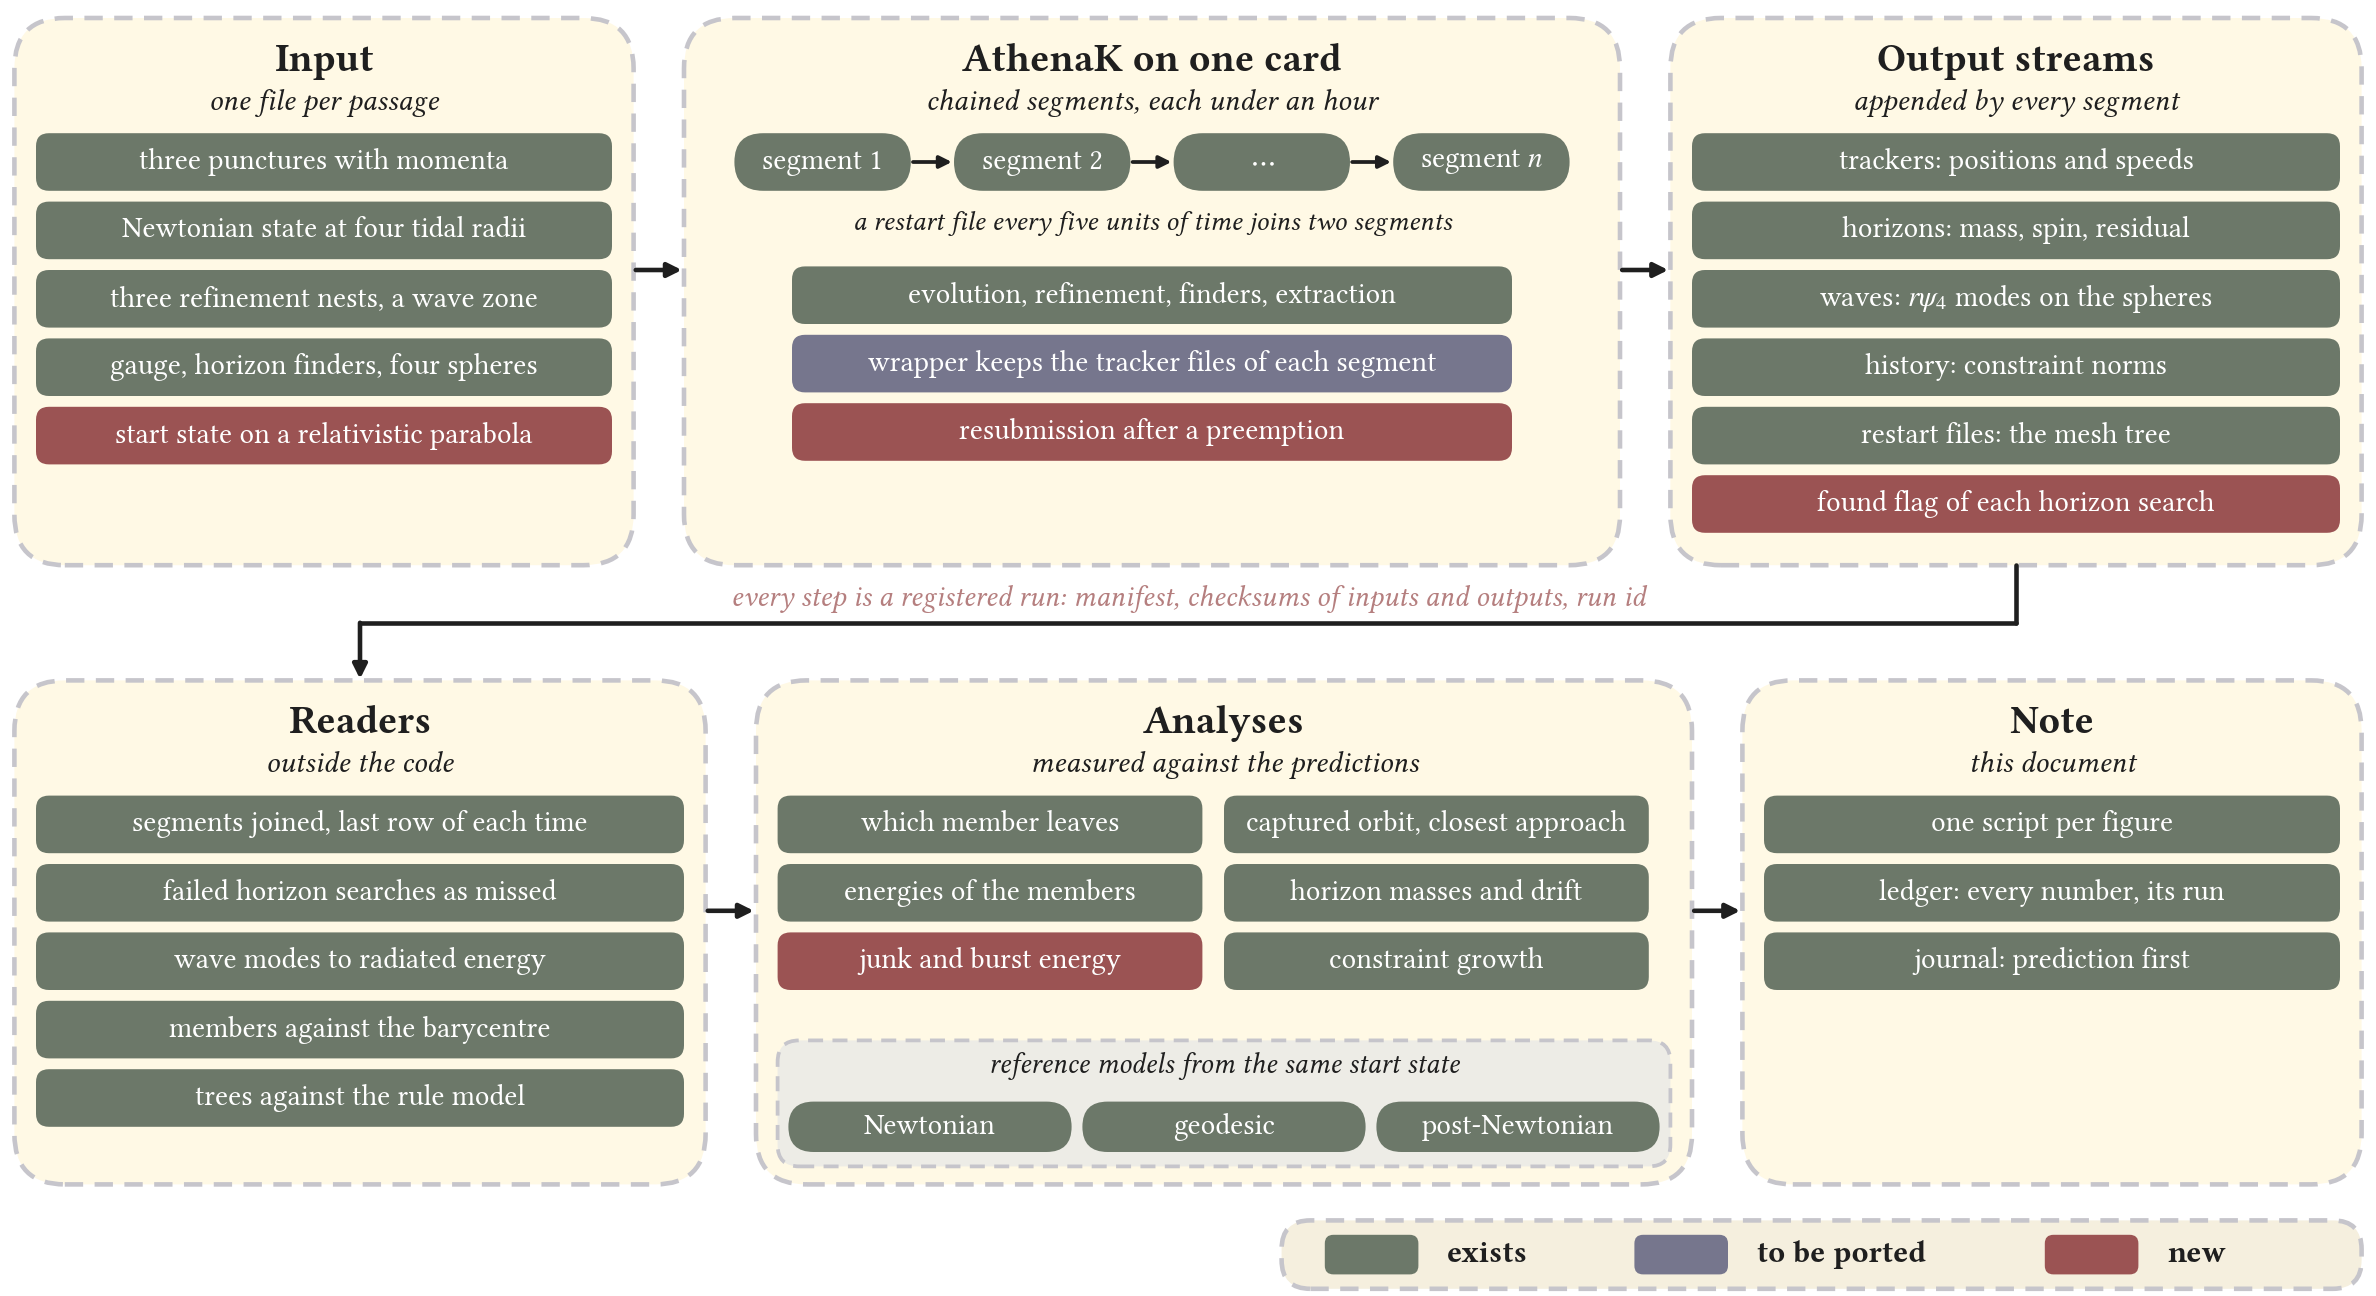
\includegraphics[width=0.94\textwidth]{schem_dataflow.png}
\caption{Data flow of one passage in full relativity. Top row: the input file, the evolution on one card in segments joined by restart files, and the output streams; bottom row: the readers, the analyses with the reference models started from the same state, and this note. Colours as in Fig.~\ref{fig:architecture}.}
\label{fig:dataflow}
\end{figure*}

\section{Reference solutions: tests and predictions}\label{sec:tests}

\subsection{Newtonian limit: the restricted problem}\label{sec:t-newton}

Figure~\ref{fig:newton} shows the restricted parabolic problem for coplanar binaries. Prograde binaries are disrupted out to a penetration factor of about two and retrograde ones out to a few tenths, the disruption probability saturates for deep encounters at the same value for both orientations, and prograde binaries reach their largest disruption probability and ejection energy near a tenth. The edges, the saturation level and the best penetration factor agree with the values printed in Ref.~\cite{Sari:2010hills}, and the curves agree with its figures to the digitising accuracy away from the edges. The retrograde edge lies slightly inside the published one; the published curve is recovered when bound binaries that end wider than a few initial separations count as disrupted, which suggests a different survival criterion in the published scan. For isotropic orientations the disruption probability and the mean energy follow the published polynomial fits \cite{Brown:2018hills} to about their stated accuracy. An independent integration of the restricted problem reproduces the prograde scan and, after wide bound binaries are followed further, the two outer retrograde points; at the two inner retrograde points a small difference remains, and the wide bound binaries there are still to be followed (Table~\ref{tab:ledger1}).

\begin{figure}
\centering
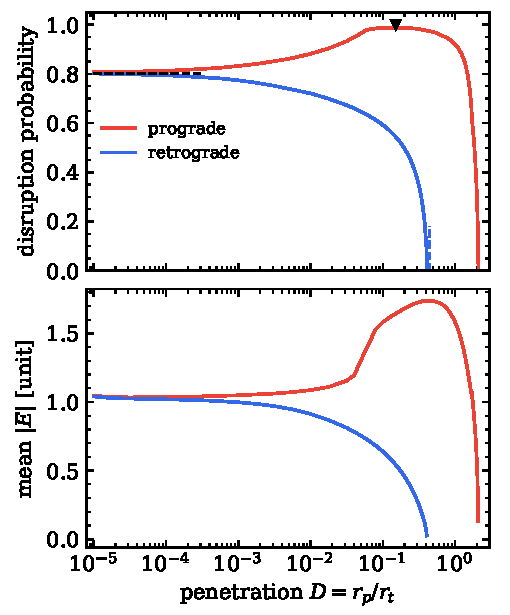
\includegraphics[width=\columnwidth]{fig_newton.pdf}
\caption{Restricted parabolic three-body problem for coplanar binaries. Top: probability that the binary is disrupted against the penetration factor; bottom: mean energy of the ejected member in the energy unit. Dashed ticks: the edges and the deep-limit saturation printed in Ref.~\cite{Sari:2010hills}; triangle: its most disruptive penetration factor.}
\label{fig:newton}
\end{figure}

\subsection{Geodesic reference in its own regime}\label{sec:t-geodesic}

Figure~\ref{fig:geodesic} repeats the scan of Ref.~\cite{Manzaneda:2024geodesic}: a binary of total mass $10^{-6}M$ sent to the black hole at penetration factors $\beta=\rt/\rp$ up to ten, every binary phase sampled, with the Newtonian and the geodesic law. For prograde binaries the two laws separate the same fraction and give nearly the same ejection speed. For retrograde binaries relativity separates binaries at smaller $\beta$, separates more of them at every $\beta$, and ejects them faster. The separation fractions agree with the published figure to its digitising accuracy, and the mean ejection speeds within a percent of the published curves. The binary stays small against the curvature radius of the black hole throughout, as the model requires. The equatorial Kerr version of the model exists; the inclined encounters in Kerr spacetime of Ref.~\cite{Zhang:2024kerr} are the next comparison \emph{(round 2: the Kerr comparison)}.

\begin{figure}
\centering
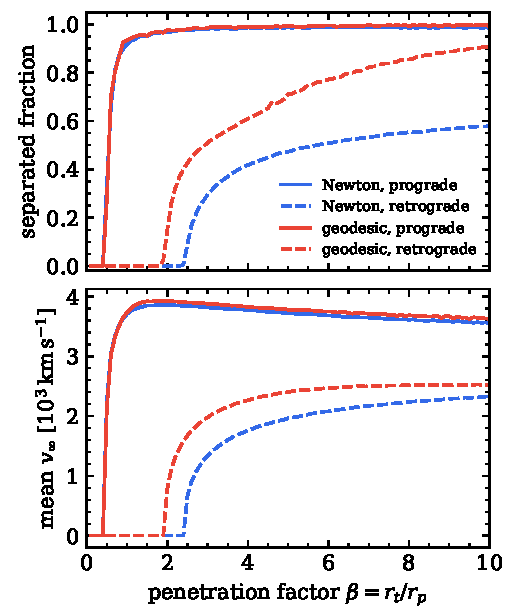
\includegraphics[width=\columnwidth]{fig_geodesic.pdf}
\caption{Geodesic reference in the set-up of Ref.~\cite{Manzaneda:2024geodesic}, binary mass $10^{-6}M$. Top: fraction of binary phases in which the binary is separated, against the penetration factor; bottom: mean ejection speed of the separated binaries. Blue: Newtonian law; red: geodesic law; solid: prograde; dashed: retrograde.}
\label{fig:geodesic}
\end{figure}

\subsection{The two references at mass ratios four and ten}\label{sec:t-scan}

Figure~\ref{fig:rpscan} applies both references to the binaries of the planned passages, at mass ratio ten with $a_b=3M$ and at four with $a_b=5M$, for pericentres from the plunge region out to about two tidal radii. The Newtonian three-body problem separates most binaries at small pericentre and fewer as the penetration factor approaches two; with the black hole held fixed it separates fewer still at the largest pericentres, so the recoil of the black hole matters at these mass ratios. In Newton's theory a member comes within $4M$ of the black hole in a sizeable fraction of the phases only at the smallest pericentre. The geodesic reference separates nearly every binary over the whole range, and in most binary phases one member crosses $2.5M$ and is swallowed; this fraction falls with the pericentre and drops below one half only at the largest pericentre at mass ratio ten.

These geodesic fractions are outputs of the model for binaries released at four tidal radii. A second agent, given the artefacts, found that the release convention and the sideways self-acceleration of a moving binary (Sec.~\ref{sec:references}) both enlarge the swallowed fraction at mass ratio ten, so the fractions frame the comparison and the full simulation supplies the prediction.

The two references therefore disagree in kind. In Newton's theory the encounter ejects one member and binds the other on a tight orbit about the black hole. In the geodesic reference, at both first passages, the member that Newton's theory binds escapes, and the one it ejects is swallowed at mass ratio ten and stays on a wide bound orbit at mass ratio four (Sec.~\ref{sec:t-passage}). The reason is the angular momentum of Sec.~\ref{sec:plunge}: after the separation one member carries less angular momentum than the marginally bound orbit, and the tight Newtonian orbit has less angular momentum than the innermost stable circular orbit of the Schwarzschild spacetime, so in relativity it plunges. Each reference captures part of these encounters: Newton's theory misses the plunge, and the geodesic model misses the recoil and holds the black hole fixed at a mass ratio of a few. The full simulation decides.

\begin{figure*}
\centering
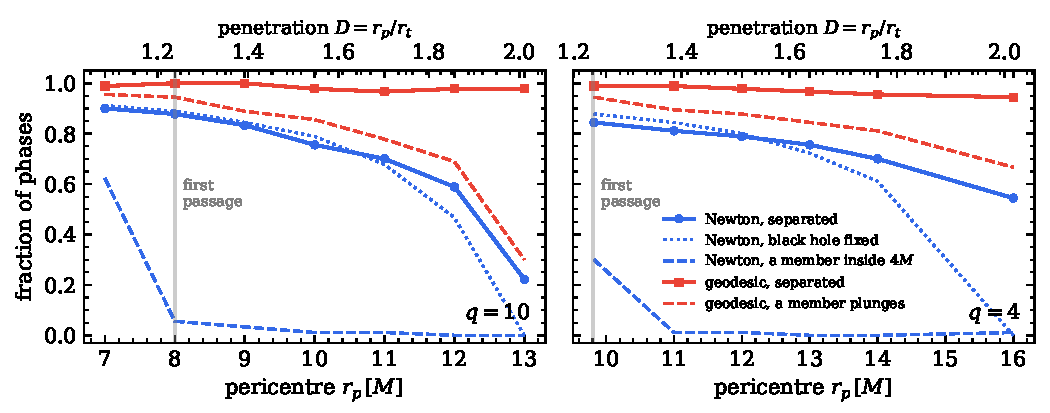
\includegraphics[width=\textwidth]{fig_rp_scan.pdf}
\caption{Fractions of binary phases against the pericentre of the centre-of-mass orbit, for the binaries of the first passages at mass ratio ten (left) and four (right), coplanar and prograde, started at four tidal radii. Blue: Newtonian three-body problem (solid: separated; dotted: separated with the black hole held fixed; dashed: a member comes inside $4M$). Red: geodesic reference (solid: separated; dashed: a member is swallowed). Grey line: pericentre of the first passage.}
\label{fig:rpscan}
\end{figure*}

\subsection{The first passages in the references}\label{sec:t-passage}

Figure~\ref{fig:passage} follows the members of the two first passages from their initial data in both references. At mass ratio four the Newtonian problem ejects the first member and binds the second on an orbit between about six and ten units of $M$, with its second pericentre inside the planned run; the geodesic reference ejects the second member and keeps the first on a wide bound orbit. The two pictures part at the pericentre passage, about a hundred units of time after the start, well inside the run. At mass ratio ten the geodesic reference swallows the first member at its first pericentre, where the Newtonian problem ejects it. The heavy black hole of the Newtonian problem moves by more than ten of its gravitational radii during the run, so the code's trajectories are read relative to its tracker. The start state of the mass-ratio-ten input, read as a relativistic test mass, turns around well inside its Newtonian pericentre or falls in (Sec.~\ref{sec:t-p1}), so that input is rebuilt from a relativistic parabola before its passage runs.

The right panels show why the energies are measured against the barycentre. The two-body energy of the escaping member with $M$ alone oscillates with the period of the captured member by a sizeable fraction of its value, while its energy against the barycentre of $M$ and the captured member settles after the encounter and stays constant. The readers of the code's output use this definition; on a Newtonian three-body run written in the code's output formats, with a restart in the middle, they recover the positions to the printed digits and the conserved energy to its value in the reference.

\begin{figure*}
\centering
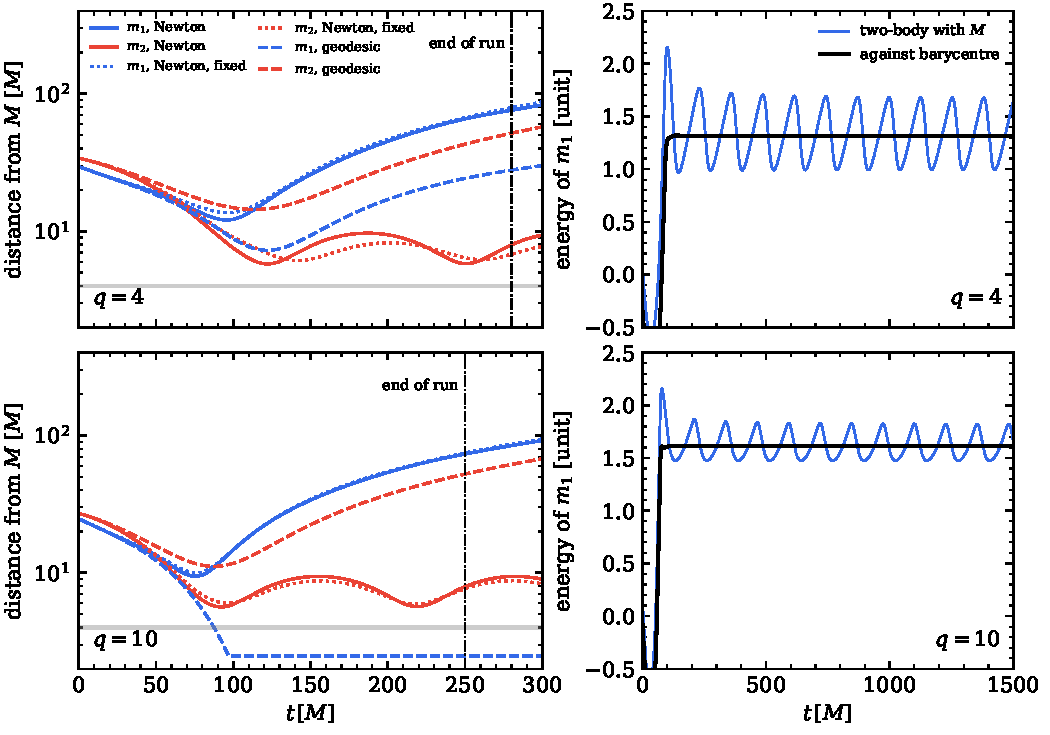
\includegraphics[width=\textwidth]{fig_passage.pdf}
\caption{The first passages in the two references, from the initial data of the full simulations at mass ratio four (top) and ten (bottom). Left: distance of each member from the heavy black hole (blue: first member; red: second) in the Newtonian problem (solid), with the black hole fixed (dotted) and in the geodesic reference (dashed; a swallowed member stops at $2.5M$); grey: $4M$; dash-dotted: end of the planned run. Right: energy of the member that Newton ejects, two-body with $M$ (blue) and against the barycentre (black).}
\label{fig:passage}
\end{figure*}

\section{Full relativity: data, members, mesh, and the first passage}\label{sec:nrtests}

\subsection{The three-black-hole data at the start}\label{sec:t-data}

Approximate initial data violate the Hamiltonian constraint, and the violation releases junk radiation when the evolution starts. For the passage the question is whether that violation or the error of the mesh dominates at the resolution of the run. Figure~\ref{fig:constraints} shows the constraint norm at the start of the passage at mass ratio four, at three resolutions, for the corrected data, for the data without the correction of the conformal factor, and for the plain sum of the punctures' conformal factors. Evaluating the closed-form residual of the same data on the same cells separates the two parts; the difference is the truncation error of the mesh.

At the resolution of the passage, $m/8$, the truncation error near the members far exceeds the data's own residual, so the corrected and uncorrected data have nearly the same norm. The correction lowers the data's own residual by more than an order of magnitude, which becomes visible at $m/16$, where the code and the closed form agree. The truncation error falls with resolution faster than the formal order of the finite differences, a pre-asymptotic rate, and away from the black holes the code reproduces the closed form at every resolution. The executable for the card gives the same norm at the start as the one for processors. The junk radiation of these data passes the extraction spheres of the first passage \emph{(round 2: the junk energy of the three-black-hole data from the spheres of the first passage)}.

\begin{figure*}
\centering
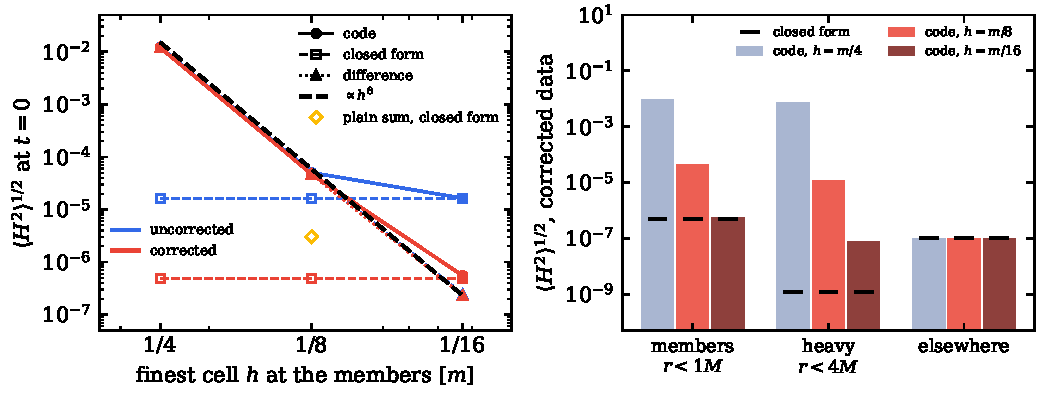
\includegraphics[width=\textwidth]{fig_constraints.pdf}
\caption{Hamiltonian constraint of the three-black-hole data of the passage at mass ratio four at the start, against the finest cell at the members. Left: volume norm for the corrected (red) and uncorrected (blue) data; circles: the code, squares: the closed form of the same data on the same cells, triangles: their difference; diamond: closed form of the plain sum. Right: the corrected data's norm by region, code (bars) and closed form (black ticks).}
\label{fig:constraints}
\end{figure*}

\subsection{A single member: gauge settling and horizon}\label{sec:t-single}

A member of the passage is a light black hole moving at about a quarter of the speed of light, in a gauge whose shift damping is set for the heavy black hole. With one damping parameter for all three black holes, the member sees in its own mass units a damping weaker by the mass ratio of the heavy black hole to the member. A single boosted puncture with the member's momentum per unit mass, evolved at the passage's resolution with the member's damping in the passage ($\eta m=0.25$) and with a damping scaled to its own mass ($\eta m=2$), shows what the member's tracker and horizon do (Fig.~\ref{fig:single}).

Under the weak damping the tracker reaches a steady fraction of the boost speed within a few member masses. Under the damping scaled to the member's mass it moves at about half the boost speed and is still accelerating when the run ends. The tracker integrates the shift at the puncture, so a slow tracker trails the black hole by a growing coordinate distance. The first horizon search finds a mass a little below the rest mass, when the horizon spans only a few cells; the next searches fail or converge to poor surfaces until the gauge has opened the coordinate horizon, and the finder then returns the rest mass of the data closely. Afterward the mass drifts slowly upward, faster under the weak damping, whose coordinate horizon is smaller. Both runs stopped early because the mesh outgrew the slots of their input (Sec.~\ref{sec:t-cost}), before the junk pulse reached the extraction spheres. A variant whose damping falls from the member's scale at the black hole to the passage's value far away has run on a card \emph{(round 2: the mass-scaled damping and the junk energy of a single member)}.

\begin{figure}
\centering
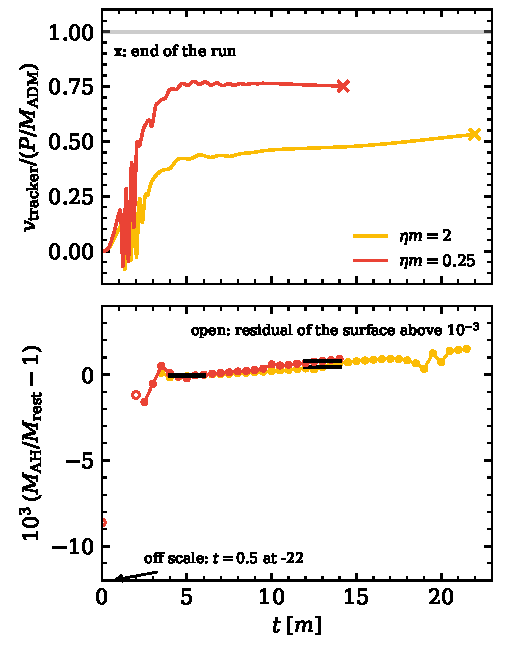
\includegraphics[width=\columnwidth]{fig_single.pdf}
\caption{A single member, a boosted puncture of mass $m$ with momentum $P=m/4$, at cells $m/8$, with weak (red) and member-scaled (yellow) shift damping. Top: tracker speed over the boost speed of the data; crosses: end of the runs. Bottom: apparent-horizon mass relative to the rest mass of the data; filled: good surfaces; black bars: window medians.}
\label{fig:single}
\end{figure}

\subsection{Mesh and cost of a passage}\label{sec:t-cost}

The mesh follows from three refinement rules: a nest of levels about each tracker, a wave zone refined out to a fixed radius, and a balance rule by which neighbouring blocks differ by at most one level. Figure~\ref{fig:tree} compares the trees stored in the restart files of the single-member runs with a model of these rules evaluated at the tracker position; they agree level by level. The model explains why those runs stopped: through the balance rule the wave zone refines every block of the root grid, and when the tracker's nest reaches the next block of a coarser level, the tree outgrows the slots of the input. Both runs stopped at that tracker position. The model now sets the slot limits of later inputs.

\begin{figure*}
\centering
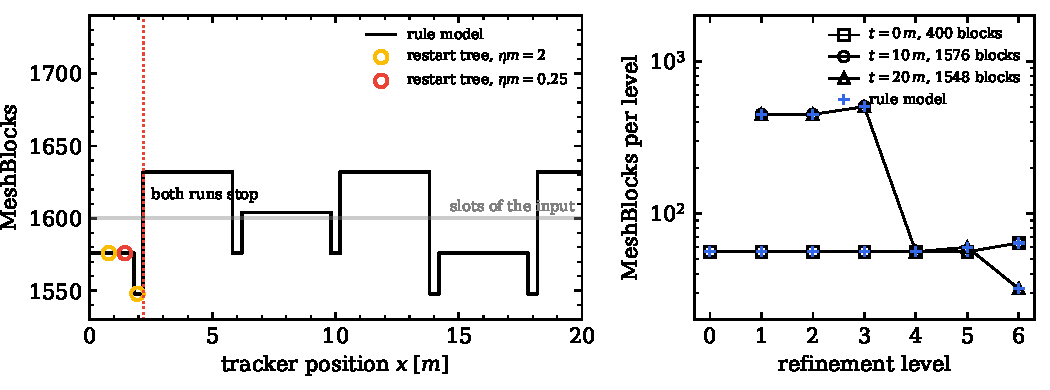
\includegraphics[width=\textwidth]{fig_tree.pdf}
\caption{Refinement tree of the single member. Left: number of mesh blocks of the model of the refinement rules against the tracker position (black), the trees in the restart files of the two runs (circles), the slots of the input (grey) and the tracker positions at which the runs stopped (dotted). Right: blocks per refinement level of three restart trees (open symbols) and of the model (crosses).}
\label{fig:tree}
\end{figure*}

Figure~\ref{fig:cost} shows the number of mesh blocks along the passage and the card time of one passage. At the resolution $m/8$ the mesh stays well below the memory of one card at both mass ratios, a passage at $q=4$ costs a fraction of the allotment to the next gate, and one at $q=10$ most of it. Doubling the resolution multiplies the cost by roughly a factor of three to four; at $q=10$ the mesh then exceeds the memory of one card, and at $q=4$ it comes close to it and above the block limit of the present input. The released code builds the same tree at the start of the $q=4$ passage as the trees used for the estimate, at both resolutions of the estimate. These numbers set the plan: the resolution study and the first scan line run at mass ratio four, and the mass ratio ten follows when two cards or larger mesh blocks are available.

\begin{figure*}
\centering
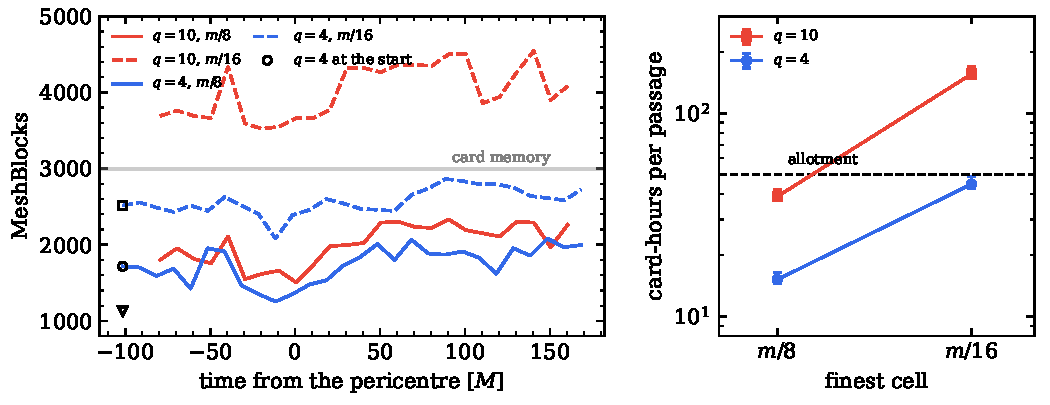
\includegraphics[width=\textwidth]{fig_cost.pdf}
\caption{Left: number of mesh blocks against time from the pericentre of the centre-of-mass orbit, at mass ratio ten (red) and four (blue) with finest cells $m/8$ (solid) and $m/16$ (dashed); open symbols: trees of the released code at the start of the $q=4$ passage with cells $m/4$, $m/8$, $m/16$ (triangle, circle, square); grey: memory of one card. Right: card-hours of one passage, median rate with the fast and slow rates as bars; dashed: allotment to the next gate.}
\label{fig:cost}
\end{figure*}

\subsection{The first passage: set-up, start state, and cost}\label{sec:t-p1}

The first passage puts the whole chain to work on the encounter about which the references disagree. It is the passage at mass ratio four of Table~\ref{tab:parameters}: corrected data, members at cells $m/8$ and the heavy black hole at $M/8$, one shift damping for all three black holes, which gives the members the weak damping of Sec.~\ref{sec:t-single}, and four extraction spheres. It runs on one card in a chain of segments (Fig.~\ref{fig:dataflow}).

The start state comes from the Newtonian three-body problem, so its centre of mass follows a Newtonian parabola. Read as a relativistic test mass about a Schwarzschild black hole, with energy and angular momentum measured in the heavy black hole's frame, the centre of mass turns around somewhat inside the Newtonian pericentre and well outside the marginally bound radius. Taken with the heavy black hole at rest, it turns around just outside the marginally bound radius, and taken about the total mass, it falls in. The start state therefore lies near the capture boundary, and the outcome depends on how the full simulation shares the motion between the three bodies; the passage itself decides. The input at mass ratio ten turns around well inside its Newtonian pericentre in the first reading and falls in under the other two.

Figure~\ref{fig:smoke} shows a short run of the passage input on one card. The tree grows slightly through the first regrids, the time per cycle stays steady, and the memory at the slot limit of the input stays below that of the card. The trackers start at the input positions; the members' trackers settle within about a dozen member masses at a steady fraction of their Newtonian speed, and the heavy black hole's tracker accelerates later and oscillates. The members' horizons are found with good surfaces from about half a unit of $M$ on, as the single member's after its gauge transient; the heavy black hole's searches fail or converge to poor surfaces in this short window, like the single member's at the same number of cells per mass, so its mass is read once its coordinate horizon has grown. The measured rate and the trees along the Newtonian track give the card time of the passage, a fraction of the allotment to the next gate.

\begin{figure*}
\centering
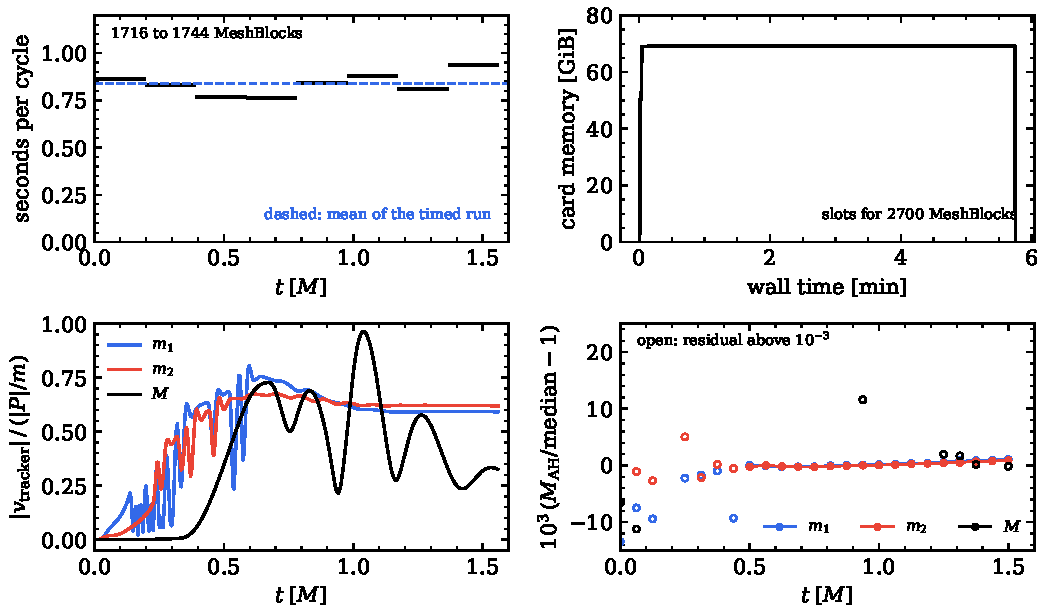
\includegraphics[width=\textwidth]{fig_smoke.pdf}
\caption{The input of the first passage for its first cycles on one card. Top left: wall-clock seconds per cycle in windows of fifty cycles (black) and their mean (dashed). Top right: card memory in use. Bottom left: tracker speed of the two members and of the heavy black hole over the speed of the data, momentum over bare mass. Bottom right: apparent-horizon masses relative to their median; open circles: surfaces with a large residual.}
\label{fig:smoke}
\end{figure*}

The prediction was recorded before the passage started (Table~\ref{tab:ledger4}). The binary is separated well inside the run, one member leaves and the other stays bound to the heavy black hole. The Newtonian problem ejects the first member and binds the second on a tight orbit whose first pericentre falls inside the run; the geodesic model ejects the second member and binds the first on a wide orbit (Sec.~\ref{sec:t-passage}). Neither member merges with the heavy black hole within the run, the tree stays below the slots of the input, and the members' horizon masses grow slowly. Which member leaves is the observable that separates the references. The passage is running \emph{(round 2: the outcome of the first passage against this prediction, the energies of both members, the horizons, and the burst; and the post-Newtonian prediction for the same start state)}.

\section{Plan and open questions}\label{sec:plan}

Figure~\ref{fig:timeline} shows the gates of the track. Gate G0 asks for the scope, the parameters, the tests and the compute estimate; its written products are complete, and the report of a fresh verifier precedes its review. Gate G1 asks that both references reproduce the literature, which they do in the Schwarzschild case \emph{(round 2: Kerr)}; that the constraint residual and the junk radiation of the three-black-hole data be quantified, of which the residual is measured (Sec.~\ref{sec:t-data}) \emph{(round 2: junk)}; and that one vacuum passage be completed, which is running (Sec.~\ref{sec:t-p1}).

Gate G2 asks that the vacuum passage converge with resolution at $q=4$, that passages at large pericentre return to both references, that a published three-black-hole encounter \cite{Campanelli:2008three} be reproduced, and that a collisionless clump at rest keep its structure much longer than a passage. Gate G3 asks for the two scan lines with three-way convergence.

Open questions, in the order they affect the next runs:
\begin{itemize}
\item Does the full simulation swallow a member where the geodesic reference does, and which member escapes? The first passage answers this for one binary phase; a phase scan in full relativity multiplies the cost of a passage by the number of phases.
\item How large are the junk radiation and the constraint violation of the approximate data compared with the burst of the passage? Approximate data can change the evolution of several black holes \cite{Galaviz:2010multiple}. At the passage's resolution the mesh dominates the violation at the start; the energy of the junk is still to be measured.
\item Which shift damping serves black holes of different masses? The single member shows that the weak damping of the passage settles the tracker quickly at the price of a faster horizon drift; a damping scaled to each mass is tested on one and two black holes and awaits a test with three.
\item The Kerr results of Ref.~\cite{Zhang:2024kerr} for inclined binaries and the post-Newtonian reference are the next comparisons of the references.
\item Objects (b) and (c) need moving equilibrium clumps and dressed black holes as initial data, from the code and from the neighbouring tracks.
\end{itemize}

\begin{figure*}
\centering
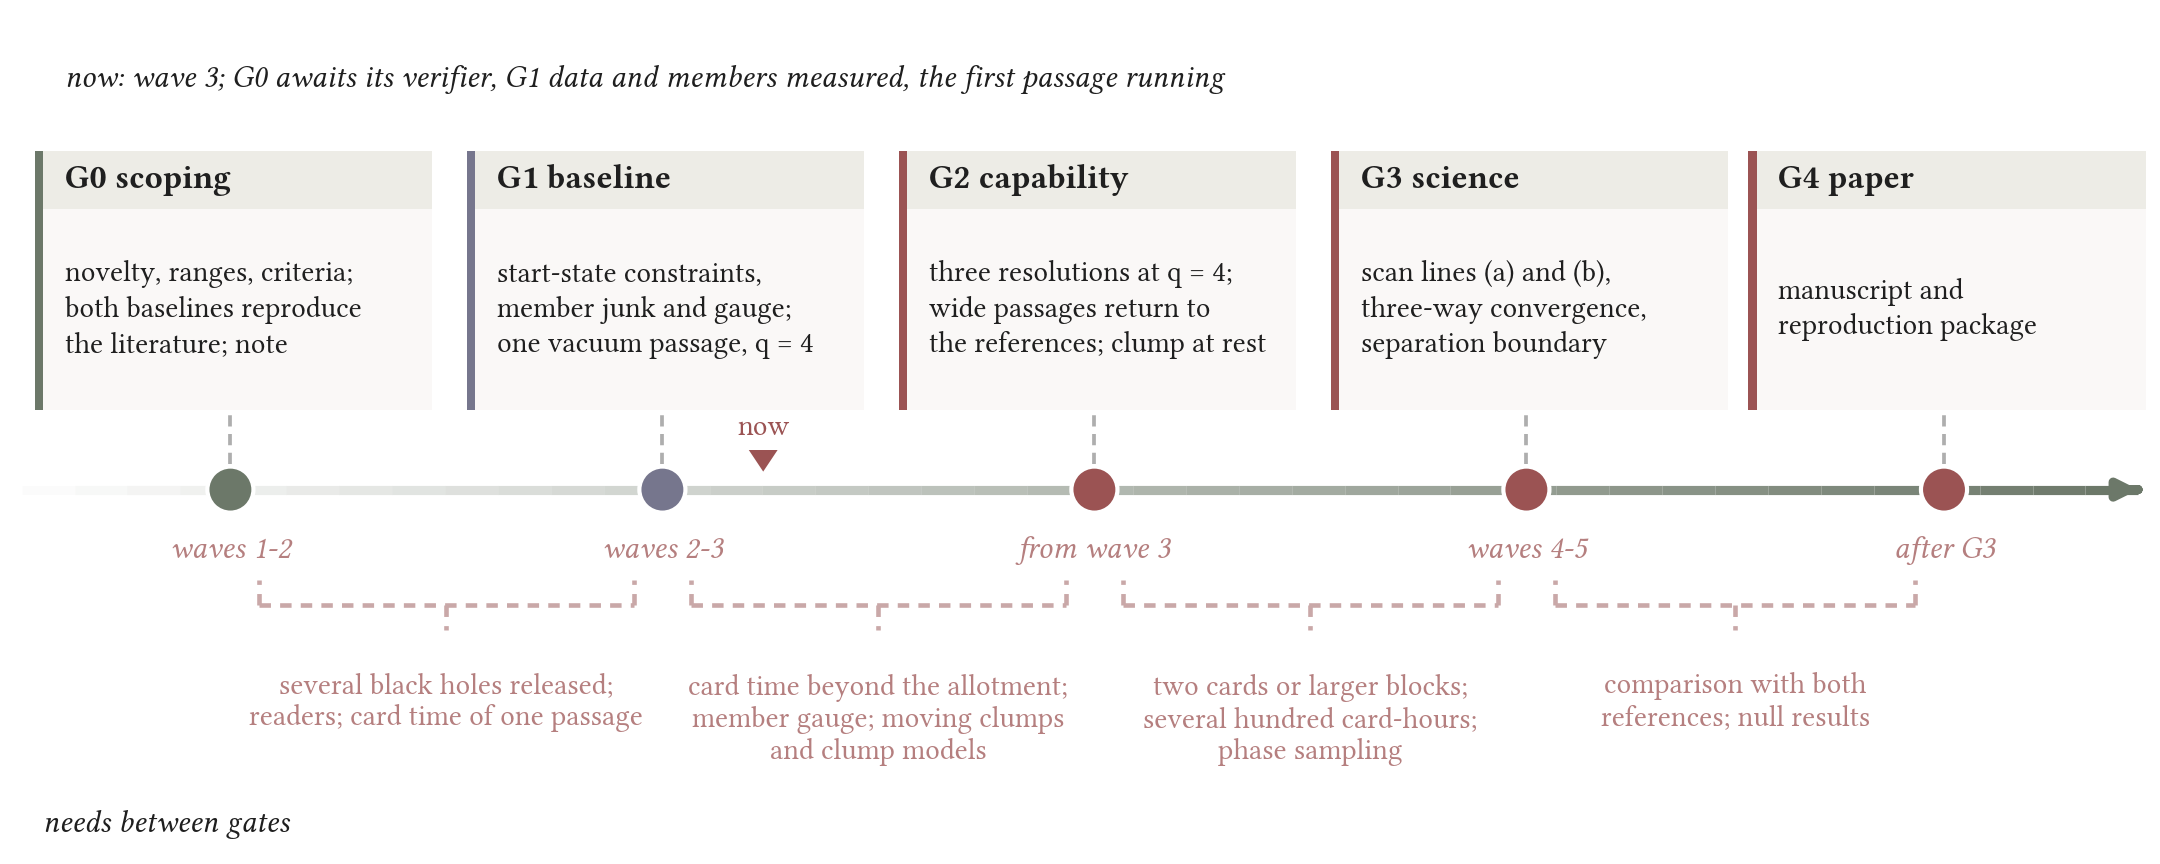
\includegraphics[width=0.92\textwidth]{schem_timeline.png}
\caption{Gates of the track. Each callout states what the gate asks; the braces below the axis name what the step to the next gate needs. The marker shows the present state.}
\label{fig:timeline}
\end{figure*}

\section{Summary}\label{sec:summary}

A binary must be wide in units of its own gravitational radius to be separated by a black hole before its centre of mass is swallowed, so at the mass ratios a full simulation reaches the encounters happen at one to two tidal radii, about ten gravitational radii from the black hole. There the binary's internal motion pushes one member below the angular momentum of the marginally bound orbit, and the two standard references part ways: Newton's theory binds that member on a tight orbit, while the geodesic model swallows it or lets the partner escape instead. Both references reproduce their published results in their own regimes, so the disagreement is physics at the edge of each model. In full relativity the baseline is in place: at the passage's resolution the mesh, and the approximate data only at finer cells, set the constraint violation at the start; a light member's tracker settles quickly under the passage's weak damping while its horizon mass creeps upward; and the mesh follows the refinement rules block by block. The first passage, at mass ratio four, starts near the relativistic capture boundary and is running on one card; it will tell which picture holds and how the energy is shared when every pair of the three bodies is relativistic.

\begin{acknowledgments}
This note, its figures and the calculations behind it were produced by large-language-model agents (Claude, Anthropic) working in the program's repository under human direction; the agents' records of predictions and outcomes are kept with the runs.
\end{acknowledgments}

\appendix

\section{Parameters of the first passages}\label{app:parameters}

Table~\ref{tab:parameters} lists the physical and simulation parameters of the two first passages. The positions and momenta of the three black holes are those of the Newtonian state at four tidal radii.

% written by scripts/ledger.py from the inputs run N1 recorded; do not edit
\begin{table}
\caption{Parameters of the two first passages (units $G=c=M=1$). Both are coplanar and prograde with nonspinning black holes and start from the Newtonian state integrated in from ten tidal radii.}
\label{tab:parameters}
\footnotesize
\begin{ruledtabular}
\begin{tabular}{p{0.46\columnwidth}ll}
Parameter & $q=4$ & $q=10$ \\ \hline
heavy black hole $M$, members $m_1=m_2$ (bare) & 1, 0.125 & 1, 0.05 \\
binary semimajor axis $a_b$, eccentricity $e_b$ at the start & 5.111, 0.033 & 3.036, 0.029 \\
tidal radius $r_t$ & 7.937 & 6.463 \\
pericentre $r_p$ and eccentricity of the centre-of-mass orbit & 9.8087, 1.00023 & 7.9965, 1.00006 \\
start distance of the centre of mass & 31.75 & 25.85 \\
domain half-width, refinement levels & 256, 10 & 204.8, 11 \\
puncture radius of refinement & 1.8 & 1.8 \\
wave extraction radii & 40, 48, 70, 90 & 40, 48, 70, 90 \\
shift damping $\eta$ (one value for all black holes) & 2.0 & 2.0 \\
end time of the run & 280 & 250 \\
\end{tabular}
\end{ruledtabular}
\end{table}


\section{Numerical ledger}\label{app:ledger}

Tables~\ref{tab:ledger1}--\ref{tab:ledger4} give every number behind this note with the registered run that produced it; the inputs of each figure and table were checked against the checksums their runs recorded (one run of the scoping stage recorded no checksums and is read as it is). The figures and tables were made in run F-20261120-222908-4ffcfba from the outputs listed; the time series of the first passages in the references come from run F-20261115-174648-25514db, which reproduces the earlier runs F-20261115-174102-ffa764f, F-hills-20261115-145251-090f5dc and F-hills-20261115-145559-a314517 in every printed digit. The single-member and smoke figures read the raw tracker, horizon and history files of runs F-20261115-173601-2fae2dc and F-20261115-174602-c6879fe and check their window means and medians against the analysis runs listed in Tables~\ref{tab:ledger3} and \ref{tab:ledger4}. Numbers quoted from the literature carry the file and line of the arXiv source, and numbers of the track's own records the file and line. The energy unit of a member follows Ref.~\cite{Sari:2010hills} (\texttt{prp.tex} lines 345--357); the consistency parameter of the geodesic reference, the binary separation over the curvature radius $(r/r_g)^{3/2}r_g$, follows Ref.~\cite{Manzaneda:2024geodesic} (\texttt{article.tex} lines 272--274).

% written by scripts/ledger.py from registered runs; do not edit
\begin{table*}
\caption{Ledger of the reference solutions. Energies in units of $(Gm_1m_2/a_b)(M/m_b)^{1/3}$; sources are registered runs or the file and line of a paper's text.}
\label{tab:ledger1}
\footnotesize
\begin{ruledtabular}
\begin{tabular}{p{0.44\textwidth}p{0.19\textwidth}p{0.29\textwidth}}
Quantity & Value & Source \\ \hline
\multicolumn{3}{l}{\emph{Scales}} \\
plunge bound $4q^{2/3}$ on $a_b/r_{gb}$, $q=10,100,1000$ & 18.57, 86.18, 400 & \texttt{\detokenize{F-hills-20261115-045435-f62d553}} \\
marginally bound radius and angular momentum (parabolic) & 4 $M$, 4 $M$ & \texttt{\detokenize{F-hills-20261115-045435-f62d553}} \\
Peters time at $a_b=30\,r_{gb}$, $q=10$ & 6328 $M$ & \texttt{\detokenize{F-hills-20261115-045435-f62d553}} \\
\multicolumn{3}{l}{\emph{Restricted Newton}} \\
last disrupting $D$, prograde & 2.085 & \texttt{\detokenize{F-hills-20261115-133222-9cb10db}} \\
deep-limit disruption probability, prograde & 0.807 & \texttt{\detokenize{F-hills-20261115-133222-9cb10db}} \\
largest ejection energy, prograde & 27.15 at $D=0.1$ & \texttt{\detokenize{F-hills-20261115-133222-9cb10db}} \\
failed integrations, prograde & 127 of 477000 & \texttt{\detokenize{F-hills-20261115-133222-9cb10db}} \\
last disrupting $D$, retrograde & 0.405 & \texttt{\detokenize{F-hills-20261115-133222-9cb10db}} \\
deep-limit disruption probability, retrograde & 0.801 & \texttt{\detokenize{F-hills-20261115-133222-9cb10db}} \\
largest ejection energy, retrograde & 1.838 at $D=1e-05$ & \texttt{\detokenize{F-hills-20261115-133222-9cb10db}} \\
failed integrations, retrograde & 92 of 477000 & \texttt{\detokenize{F-hills-20261115-133222-9cb10db}} \\
largest disruption probability (prograde) & 0.988 at $D=0.16$ & \texttt{\detokenize{F-hills-20261115-133222-9cb10db}} \\
printed: last disrupting $D$; largest energy; deep limit; best $D$ & 2.1/0.44; 27.3/1.8; about 0.8; 0.15 & arXiv:0911.1136 prp.tex:735-738, 846-849, 854 \\
against the digitised curve: median, largest $|\Delta P|$, prograde & 0.0014, 0.037 at $D=2.07$ & \texttt{\detokenize{F-hills-20261115-132703-0bfc352}} \\
retrograde, bound binaries wider than $3.5\,a_b$ counted as disrupted: largest $|\Delta P|$ against the digitised curve, last disrupting $D$ & 0.0088, 0.445 & \texttt{\detokenize{F-hills-20261115-132942-2f7ad7f}} \\
against the digitised curve: largest $|\Delta P|$, retrograde & 0.21 at $D=0.418$ & \texttt{\detokenize{F-hills-20261115-132703-0bfc352}} \\
isotropic orientations, $D\le1$: largest fractional deviation from the published fit, probability and mean energy & 0.015, 0.017 (512 orientations $\times$ 64 phases) & \texttt{\detokenize{F-hills-20261115-133200-05ee76a}} \\
printed: plateau of the isotropic probability; accuracy of the fits for $D\lesssim1$ & about 0.88; 1\% & arXiv:1804.02911 mnras.tex:368, 377, 440 \\
independent code, nine points: largest $|\Delta P|$, $|\Delta E|/E$ & 0.021, 0.079 (retrograde $D=0.38$) & \texttt{\detokenize{F-hills-20261115-145246-090f5dc}} \\
the same at retrograde $D=0.3, 0.38$, wide binaries followed on & 0.0013, 0.0035 & \texttt{\detokenize{F-hills-20261115-145544-a314517}} \\
\multicolumn{3}{l}{\emph{Geodesic baseline}} \\
encounters of the scan & 160000 & \texttt{\detokenize{F-hills-20261115-142554-c10b371}} \\
retrograde onset of separation in $\beta$ (geodesic, Newton) & 1.9, 2.5 & \texttt{\detokenize{F-hills-20261115-142554-c10b371}} \\
separated fraction at $\beta=3$ (N pro, N retro, G pro, G retro) & 0.98, 0.295, 0.985, 0.51 & \texttt{\detokenize{F-hills-20261115-142554-c10b371}} \\
separated fraction at $\beta=10$ (N pro, N retro, G pro, G retro) & 0.985, 0.58, 0.993, 0.91 & \texttt{\detokenize{F-hills-20261115-142554-c10b371}} \\
against the figure of arXiv:2404.16270: largest $|\Delta|$ of the fraction & 0.0225 & \texttt{\detokenize{F-hills-20261115-142554-c10b371}} \\
the same, mean $v_\infty$ (relative) & 0.0073 & \texttt{\detokenize{F-hills-20261115-142554-c10b371}} \\
largest $a_b/R_{\rm curv}$ of a bound binary at $\beta=10$ & 0.0056 & \texttt{\detokenize{F-hills-20261115-142554-c10b371}} \\
\end{tabular}
\end{ruledtabular}
\end{table*}

\begin{table*}
\caption{Ledger of the pericentre scan, the first passages and the cost. Fractions are over the sampled binary phases; card-hours are the median rate with the fast and slow rates in parentheses.}
\label{tab:ledger2}
\footnotesize
\begin{ruledtabular}
\begin{tabular}{p{0.44\textwidth}p{0.19\textwidth}p{0.29\textwidth}}
Quantity & Value & Source \\ \hline
\multicolumn{3}{l}{\emph{Pericentre scan}} \\
$q=10$, $r_p=7$: Newton sep., inside $4M$; geodesic sep., plunge & 0.9, 0.62; 0.99, 0.96 & \texttt{\detokenize{F-hills-20261115-145915-71abf93}} \\
$q=10$, $r_p=8$: the same & 0.88, 0.056; 1, 0.94 & \texttt{\detokenize{F-hills-20261115-145915-71abf93}} \\
$q=10$, $r_p=13$: the same & 0.22, 0; 0.98, 0.3 & \texttt{\detokenize{F-hills-20261115-145915-71abf93}} \\
$q=4$, $r_p=9.82$: Newton sep., inside $4M$; geodesic sep., plunge & 0.84, 0.3; 0.99, 0.94 & \texttt{\detokenize{F-hills-20261115-145915-71abf93}} \\
$q=4$, $r_p=16$: the same & 0.54, 0.011; 0.94, 0.67 & \texttt{\detokenize{F-hills-20261115-145915-71abf93}} \\
\multicolumn{3}{l}{\emph{First passages}} \\
$q=4$: energy unit $(m_1m_2/a_b)q^{1/3}$ & 0.004961 $M$ & \texttt{\detokenize{F-20261115-174648-25514db}} \\
$q=4$, Newton: ejected member, energy (barycentric), its spread after $t=300M$ & $m_1$, 1.3119, 0.00015 & \texttt{\detokenize{F-20261115-174648-25514db}} \\
$q=4$, Newton: two-body energy of the same member with $M$, range & 0.9887 to 1.723 & \texttt{\detokenize{F-20261115-174648-25514db}} \\
$q=4$, Newton: captured member, energy, closest approach & $m_2$, -1.627, 5.777 $M$ & \texttt{\detokenize{F-20261115-174648-25514db}} \\
$q=4$, geodesic: ejected member and energy; other member & $m_2$, 0.9703; bound, -0.5, first pericentre 7.262 $M$ & \texttt{\detokenize{F-20261115-174648-25514db}} \\
$q=4$, Newton with $M$ fixed: ejected energy, closest approach of the other & 1.835, 6.107 $M$ & \texttt{\detokenize{F-20261115-174648-25514db}} \\
$q=10$: energy unit $(m_1m_2/a_b)q^{1/3}$ & 0.001795 $M$ & \texttt{\detokenize{F-20261115-174648-25514db}} \\
$q=10$, Newton: ejected member, energy (barycentric), its spread after $t=300M$ & $m_1$, 1.6127, 3.2e-05 & \texttt{\detokenize{F-20261115-174648-25514db}} \\
$q=10$, Newton: two-body energy of the same member with $M$, range & 1.474 to 1.845 & \texttt{\detokenize{F-20261115-174648-25514db}} \\
$q=10$, Newton: captured member, energy, closest approach & $m_2$, -1.845, 5.641 $M$ & \texttt{\detokenize{F-20261115-174648-25514db}} \\
$q=10$, geodesic: ejected member and energy; other member & $m_2$, 1.159; plunges at $t=97.1M$ & \texttt{\detokenize{F-20261115-174648-25514db}} \\
$q=10$, Newton with $M$ fixed: ejected energy, closest approach of the other & 1.887, 5.862 $M$ & \texttt{\detokenize{F-20261115-174648-25514db}} \\
$q=4$: reproduces the earlier run in every printed digit (ejected energy) & 1.31187 & \texttt{\detokenize{F-20261115-174102-ffa764f}} \\
$q=4$, Newton: displacement of the heavy black hole by the end of the run & 13.3 $M$ at $t=280M$ & \texttt{\detokenize{F-20261115-174102-ffa764f}} \\
readers on a synthetic three-body run: checks passed & 10 of 10 & \texttt{\detokenize{F-20261115-173821-b2c969a}} \\
$q=10$: captured orbit of Newton ($a$, $e$, pericentre) & 7.55, 0.247, 5.68 $M$ & \texttt{\detokenize{F-hills-20261115-145251-090f5dc}} \\
\multicolumn{3}{l}{\emph{Mesh and cost}} \\
$q=10$, $m/8$: MeshBlocks start, largest, mean; card-hours (240 $M$) & 1800, 2332, 2006; 38.9 (37-42.3) & \texttt{\detokenize{F-hills-20261115-131348-634fb86}} \\
$q=10$, $m/16$: MeshBlocks start, largest, mean; card-hours (240 $M$) & 3690, 4544, 4019; 156 (149-170) & \texttt{\detokenize{F-hills-20261115-131348-634fb86}} \\
$q=10$, $m/16$, small radius: MeshBlocks start, largest, mean; card-hours (240 $M$) & 2654, 2934, 2574; 99.4 (94.7-108) & \texttt{\detokenize{F-hills-20261115-131348-634fb86}} \\
$q=4$, $m/8$: MeshBlocks start, largest, mean; card-hours (270 $M$) & 1716, 2080, 1744; 15.2 (14.5-16.5) & \texttt{\detokenize{F-hills-20261115-131933-907e5fe}} \\
$q=4$, $m/16$: MeshBlocks start, largest, mean; card-hours (270 $M$) & 2514, 2864, 2568; 44.8 (42.7-48.7) & \texttt{\detokenize{F-hills-20261115-131933-907e5fe}} \\
$q=4$, $m/16$, small radius: MeshBlocks start, largest, mean; card-hours (270 $M$) & 2416, 2654, 2348; 40.9 (39-44.6) & \texttt{\detokenize{F-hills-20261115-131933-907e5fe}} \\
rate, MeshBlock-cycles per second (median, slow, fast) & 2201, 2022, 2310 & \texttt{\detokenize{F-hills-20261115-131348-634fb86}} \\
$q=4$ input at the start, release executable: $m/4$, $m/8$, $m/16$ & 1128, 1716, 2514 & \texttt{\detokenize{F-20261115-173543-29e87e8}} \\
card memory, MeshBlock slots & about 3000 & coord/INTERFACES/multi\_puncture.md:229-230 \\
\end{tabular}
\end{ruledtabular}
\end{table*}


\bibliography{references}

\end{document}
